% set home directory
\providecommand{\homedir}{..} 
% load the preamble of main.tex by subfiles
\documentclass[\homedir/main.tex]{subfiles}
% ##############################################################################
\begin{document}
% set chapter numbering to work correctly even when separate compilation using subfile
\setcounter{chapter}{4}
\chapter{評価実験}\label{chap:experiment}
本研究では,\cref{chap:methods}で述べた手法を評価するためにアンケートを実施した.
そこで,本章ではまず\cref{sec:experimental_details}で実施したアンケートの内容を述べる.
その後,\cref{sec:experimental_results}で得たアンケート結果を述べる.
本章の最後に,\cref{sec:consideration}では
\cref{sec:experimental_results}で述べた結果を踏まえて考察を述べる.

% ##############################################################################
\section{アンケート内容}\label{sec:experimental_details}
本研究では,提案手法の評価のために同研究室の学生および情報処理領域の学生を対象に
アンケート形式の調査を実施し,最終的に計15人から回答を得た.
実施したアンケートは5つのセクションで構成されており,
各セクションは次のような意図を持って設計した.

\begin{enumerate}[label=\textbf{セクション\arabic*.}]
    \setlength{\leftskip}{3.0cm}
    \item コンテンツの文字種による影響の調査
    \item エフェクトのスタイルによる影響の調査その1
    \item 歪みのスタイルを指定する文字列画像の文字種による影響の調査
    \item エフェクトのスタイルによる影響の調査その2
    \item 歪みのスタイルによる影響の調査
\end{enumerate}

但し,これらの各セクションの意図は回答者に伏せた状態でアンケートを実施した.

実施したアンケートは,提案手法を用いてデザイン文字列を作成した際の入出力の組み合わせを
次の\cref{fig:io_compilation_eg}に示すような形式で纏めた画像と,
その画像に関する選択式の設問,自由記述式の設問のセットが繰り返される形式となっている.

\begin{figure}[h]
    \centering
    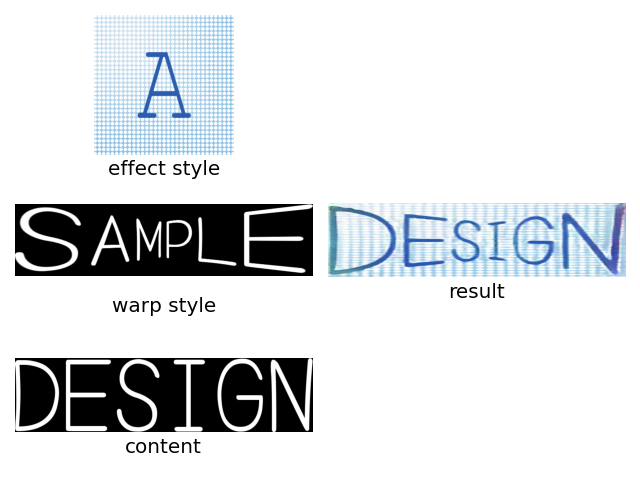
\includegraphics[keepaspectratio, width=0.6\linewidth]{input_output_compilation_example.png}
    \caption{回答者に提示した入出力の組み合わせを示す画像の例}
    \label{fig:io_compilation_eg}
\end{figure}

この\cref{fig:io_compilation_eg}は左半分に配置された画像が提案手法で用いる入力画像であり,
右のresultがそれらの入力画像から作成された出力画像である.
そして\cref{fig:io_compilation_eg}の左半分の画像は上から順に,
effect styleがエフェクトのスタイルを指定する文字デザインを意味し,
warp styleが歪みのスタイルを指定する文字列画像を意味し,
contentがコンテンツ画像を意味している.

選択式の設問は,いずれもその設問に対応する\cref{fig:io_compilation_eg}の形式の画像を見て,
\begin{enumerate}[label=\textbf{項目\arabic*:}]
    \setlength{\leftskip}{0.8cm}
    \item resultの色や効果はeffect styleと似ている
    \item resultの文字列の歪みはwarp styleと似た形状である
    \item resultの文字列はcontentの文字列と同じ文字と分かる
    \item resultのデザイン文字列は上手く生成されている
\end{enumerate}
の4つの項目それぞれについて
「全く当てはまらない」
「あまり当てはまらない」
「どちらともいえない」
「やや当てはまる」
「とても当てはまる」
の五段階で評価するものである.
\newpage
なお,アンケートを集計する際にはこの選択式の設問の回答を
\begin{enumerate}
    \item 全く当てはまらない
    \item あまり当てはまらない
    \item どちらともいえない
    \item やや当てはまる
    \item とても当てはまる
\end{enumerate}
というように1から5の整数値に対応づけて数値として扱うとする.

自由記述式の設問は,回答者がその設問に対応する\cref{fig:io_compilation_eg}の形式の画像を見て,
\begin{itemize}
    \item 画像のデザイン文字列が特に上手く生成できていると感じたとき
    \item 画像のデザイン文字列が特に印象に残ったとき
    \item 画像のデザイン文字列が特に生成に失敗していると感じたとき
\end{itemize}
のような場合やその他に意見があるとき,自由に意見を記述してもらう設問である.

また,各セクションの設問数と説明を表に纏めたものが次の\cref{tab:questionnaire_results}である.

\begin{table}[h]
    \centering
    \caption{各セクションについて}
    \begin{tabular}[t]{ccc}
        \toprule
        セクション & 設問数 & セクションの説明                           \\
        \midrule
        1     & 3   & contentの文字種に英大文字,英小文字,漢字の3つを試した    \\
        2     & 5   & effect styleを5種類試した                \\
        3     & 3   & warp styleの文字種に英大文字,英小文字,漢字の3つを試した \\
        4     & 5   & effect styleを5種類試した                \\
        5     & 4   & warp styleの歪み方を4種類試した              \\
        \bottomrule
    \end{tabular}
    \label{tab:explanation_about_each_section}
\end{table}


最後に,本アンケートを作成するのに用いたデータについて述べる.
本アンケートのeffect styleはセクション2のもののみ
先行研究\cite{Yang2019TETGAN}のデータセット中の画像を使用しており,
その他のセクションのeffect styleは
先行研究\cite{typography2019}のデータセット中の画像を使用している.
また,warp styleやcontentの文字列のフォントには「Yomogi」
\footnote{
    Copyright 2020 The Yomogi Project Authors
    (https://github.com/satsuyako/YomogiFont), all rights reserved.
}
を使用している。
\newpage

% ##############################################################################
\section{アンケート結果}\label{sec:experimental_results}
\cref{sec:experimental_details}に示したアンケートのうち選択式の設問の回答を,
項目ごとに全回答者の平均値を取って表にまとめたものが次の\cref{tab:questionnaire_results}である.

\begin{table}[h]
    \centering
    \caption{アンケートの結果}
    \begin{tabular}[t]{ccccccc}
        \toprule
        設問    & 項目1         & 項目2         & 項目3         & 項目4         & 全項目         \\
        \midrule
        1 - 1 & 4.533333333 & 4.6         & 4.733333333 & 4.533333333 & 4.6         \\
        1 - 2 & 4.066666667 & 3.066666667 & 3.4         & 3.066666667 & 3.4         \\
        1 - 3 & 4           & 3           & 2.533333333 & 2.6         & 3.033333333 \\
        \hline
        2 - 1 & 4.266666667 & 4.666666667 & 4.8         & 4.4         & 4.533333333 \\
        2 - 2 & 4.2         & 4.533333333 & 4.8         & 4.333333333 & 4.466666667 \\
        2 - 3 & 3.933333333 & 4.533333333 & 4.733333333 & 4.066666667 & 4.316666667 \\
        2 - 4 & 3.133333333 & 4.2         & 4.733333333 & 3.733333333 & 3.95        \\
        2 - 5 & 3.666666667 & 4.333333333 & 4.8         & 4           & 4.2         \\
        \hline
        3 - 1 & 4.2         & 3           & 4.266666667 & 3.4         & 3.716666667 \\
        3 - 2 & 4.466666667 & 4.2         & 4.666666667 & 4.133333333 & 4.366666667 \\
        3 - 3 & 3.466666667 & 2.133333333 & 1.6         & 1.533333333 & 2.183333333 \\
        \hline
        4 - 1 & 3.066666667 & 4.333333333 & 4.8         & 3.6         & 3.95        \\
        4 - 2 & 4.4         & 4.733333333 & 4.8         & 4.533333333 & 4.616666667 \\
        4 - 3 & 4.066666667 & 4.666666667 & 4.733333333 & 4.133333333 & 4.4         \\
        4 - 4 & 2.8         & 4.266666667 & 4.333333333 & 3.133333333 & 3.633333333 \\
        4 - 5 & 2.8         & 4.533333333 & 4.6         & 3.4         & 3.833333333 \\
        \hline
        5 - 1 & 4.333333333 & 4.6         & 4.8         & 4.466666667 & 4.55        \\
        5 - 2 & 4.533333333 & 4.666666667 & 4.866666667 & 4.666666667 & 4.683333333 \\
        5 - 3 & 4.333333333 & 4.6         & 4.266666667 & 4.066666667 & 4.316666667 \\
        5 - 4 & 4.2         & 3           & 4.6         & 3.2         & 3.75        \\
        \bottomrule
    \end{tabular}
    \label{tab:questionnaire_results}
\end{table}


% ##############################################################################
\section{考察}\label{sec:consideration}
\cref{tab:questionnaire_results}のアンケート結果を見るとほどんどの項目で4以上の評価となっているため,
提案手法を用いたデザイン文字列の作成は概ね成功したといえる.
しかし,設問3-3の評価が極端に悪い.
これは歪みのスタイルを指定する文字列画像に漢字を用いたため,
歪みの転写が失敗したことが原因だと考えられる.

% ##############################################################################
\printBibForSubfiles
\end{document}